\section{Super resolution} \label{sec:SR}

    Single image Super-Resolution (SR) is the task of increasing the resolution of a given image as well as sharpening its content by predicting the high-frequency component and the missing information

    Super resolution refers to an image processing process of recovering a corresponding high-resolution image from a low-resolution version of it, with applications that range from natural images \cite{zeyde2010single}, \cite{martin2001database} to satellite \cite{valsesia2021permutation} and medical imaging \cite{bashir2021comprehensive}. SR remains a challenging task in computer vision because it is considered an ill-posed problem: several HR images can generate exactly the same LR image. 

       \begin{figure}[h!]
            \centering
            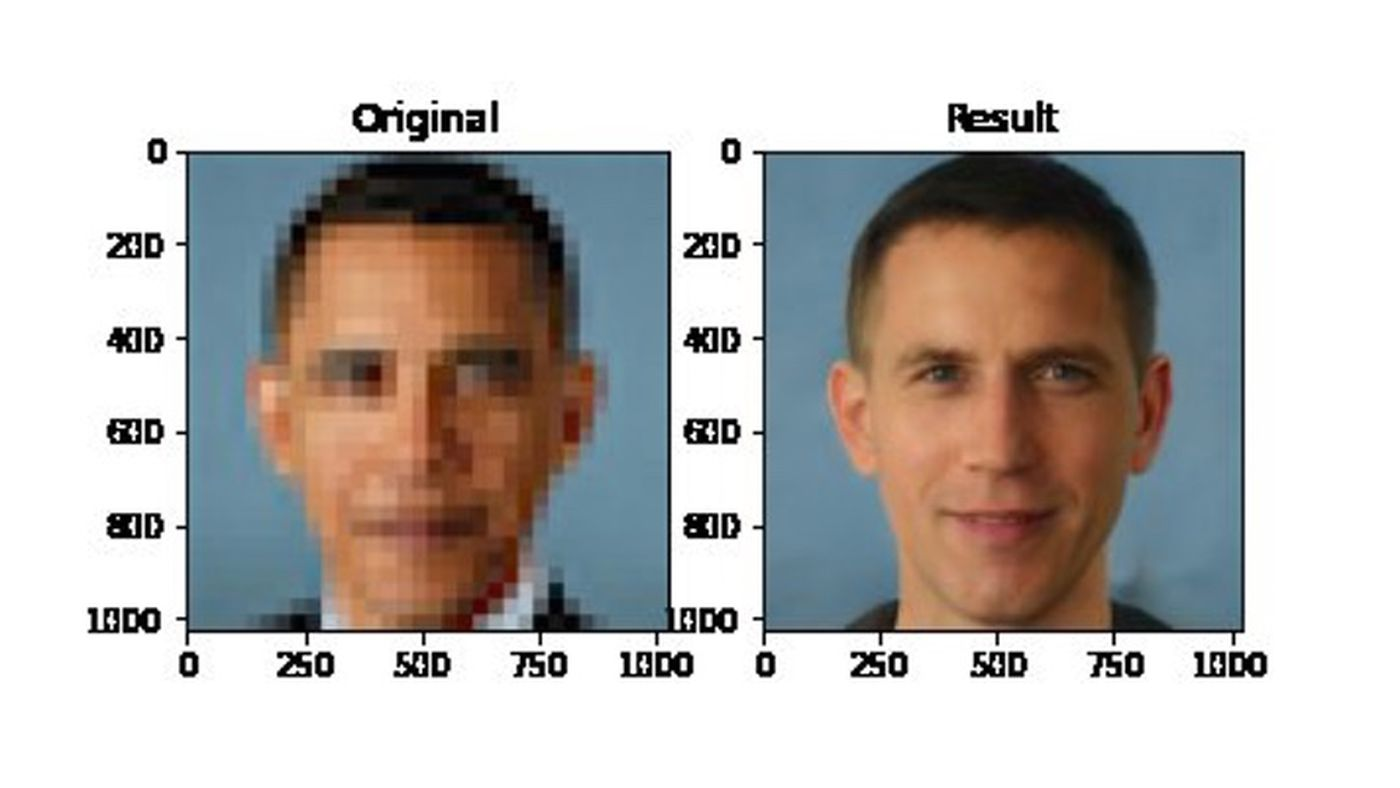
\includegraphics[scale=0.2]{Includes/2-SR-ill-posed.jpg}
            \caption{Example of super resolution as an ill posed problem. A blurry picture of Barack Obama can be generated from an HR image of another person.}
            \label{fig:2-SR-ill-posed}
        \end{figure}
    
    Depending on the different number of low-resolution inputs, image super resolution reconstruction can be divided into single-image or multi-image. ASDFAGDSGADFSGAFSFAD

    Traditional interpolation-based methods for upsampling images were the first type of algorithms used for super resolution. The most common techniques are nearest-neighbor, bilinear and bicubic interpolation. Nearest-neighbor interpolation is the most straightforward algorithm, as the interpolated value is based on its nearest pixel values.  While this method requires almost no calculations, the results are usually blocky because there are no interpolated smooth transitions.
    Bilinear and bicubic interpolation produces smoother transitions using linear or cubic interpolation in both axes. Bilinear interpolation needs a receptive fields of 2x2 and is usually faster, bicubic needs a receptive field of 4x4. THe latter is the most common baseline to understand the improvement of a super resolution network. 

    

\begin{itemize}
    \item what is super resolution?
    \item Interpolation based vs reconstruction-based vs learning-based
\end{itemize}

    \subsection{Single-Image Super Resolution}

        In a typical SISR framework, the LR image $I^{LR}$ is modeled as follows:
    
        \begin{equation}
            I^{LR} = ( I^{HR} \ast k) \downarrow_s + \ n
        \end{equation}
    
        Where $I^{HR} \ast k$ is the convolution between a blurring kernel $k$ and the unknown  HR image  $I^{HR}$, $\downarrow_s$ is the downsampling operator with scaling factor $s$ and $n$ is a noise term. Super resolution objective is to solve this equation and obtain $I^{HR}$ which as stated before, is an extremely ill-posed problem. Super resolution was first proposed in the 1960s, while the first use of multiple images dates of 1989. Machine learning was used for the first time in 2000. Deep learning appears as a branch of machine learning, emphasizing the use of multi-layer neural network cascade for feature exctraction and representation. The rise of the technology wave around 2010 changed the way of solving problems in different branches. Instead of piecing together individual functional modules to form a system, the focus is to optimize parameters by global training after the whole system is designed, what is called end-to-end training. 
        \subsubsection{SR Resnet}
    \subsection{Multi-Image Super Resolution}

        Multi-Image Super-Resolution (MISR) is the task of yielding HR images by fusing multiple LR observations of the same scene, which allows the achievement of higher reconstruction accuracy than relying on only one image. The development of this approach progressed at a slower pace due to the extesive pre-processing requirements imposed on the input, as this algorithms have a high sensibility to the input variability and their proper co-registration.  

        When the input images are of the same nature, but taken at different points in the temporal dimension, the problem is often called multi-image super resolution. On the other hand, when the images are taken at the same time but they come from different sensors and show different spectral bands, it is called multi-spectral super resolution, which will be further discussed. 

        In 2019, the European Space Agency (ESA) organized an SR challenge  \cite{martens2019superresolution} based on real-world scenes acquired by the PROBA-V satellite, each of which contains an HR image (100m GSD) coupled with at least nine LR images that are not perfectly co-registered and they may be taken months apart. This challenge, with a not synthetically generated HR-LR image pairs, fostered a new generation of model architectures that are able to fuse the multiple LR images to create better reconstructions.

        \begin{figure}[h!]
            \centering
            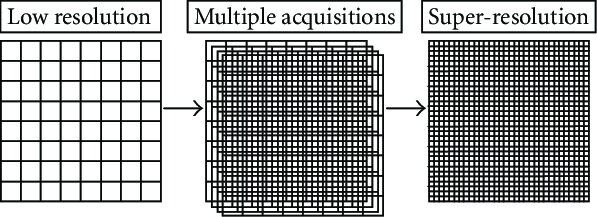
\includegraphics[scale=1.5]{Includes/2-MISR.jpeg}
            \caption{Multi-image super resolution algorithms combine multiple low-resolution image acquisitions into a high-resolution image. Source: \cite{MISR2007}}
            \label{fig:2-MISR}
        \end{figure}
        
        \subsubsection{Multi-spectral super resolution}

        Also Referred to as "hyper-spectral super resolution" in the literature, The term "Multi-Spectral" emphasizes the use of multiple spectral bands, in contrast with the multi-image approach detailed previously. While the concept bears similarities to MISR, the key distinction lies in MSSR's use of a single scene captured with different spectral bands, as opposed to multiple images, to reconstruct a superior, super-resolved image.

        In the context of MSSR, each spectral band, corresponding to a specific wavelenght range, provides unique information about the observed scene. Some of the spectral bands yield better resolution because of their physical properties and the costs related to their sensors. Using this higher resolution bands to increase the detail in the lower bands seems like a resaonable approach.

        Traditional pan-sharpening algorithms could be considered as deterministic MSSR  algorithms. It is usually used to increase the resolution of a multi-spectral RGB image using the panchromatic band. The overlap between the wavelengths of both wavelength ranges makes this algorithm straightforward. However, it is ill-suited for Thermal Infrared (TIR) data due to the disjointed spectral domains of the visible and TIR bands. In \cite{myself2023}, A deep learning is trained assuming the presence of common information between low-resolution LWIR images and their higher resolution RGB counterparts, with the objective of creating a super-resolved product in the LWIR band by an effective fusion. This improved image retains the essential thermal information, while simultaneously incorporated enhanced spatial resolution details captured from the visible bands. 

        \subsubsection{Importance of interframe correlation}
        \subsubsection{RAMS}
    \subsection{The domain gap problem} \label{subsec:domaingap}
 
        SR is a supervised problem, the super resolved image is compared to the HR ground truth and the pixel-by-pixel differences drive the gradients of the neural network to minimize the loss, in a fully supervised manner. 
        Additionally, deep learning based SR methods are known to consume large quantities of training data.
        Most of the research in the field of SR is conducted by artificially producing HR-LR pairs by downscaling the HR images with known kernels, such as bicubic.
        However, this is rarely the case when using "non-ideal", real world images.
        In spite of their success on synthetic datasets, the poor generalization capacity of the trained SR networks limits their application in real scenarios, leading to blurry images and strange artifacts in the SR results \cite{lugmayr2020ntire}.



        The domain gap problem is the difference between the training data and the real-world data. The training data is usually generated synthetically, using bicubic downsampling, which is a very simple degradation model. However, real-world degradations are usually too complex to be modelled with an explicit combination of multiple degradation types, as shown in Fig.3(c). Therefore, implicit modelling attempts to circumvent the explicit modelling function. Instead, it defines the degradation process f implicitly through data distribution, and all the existing approaches with implicit modelling require an external dataset for training. Typically, these methods utilize data distribution learning with Generative Adversarial Network (GAN) [16] to grasp the implicit degradation model possessed within training dataset, like CinCGAN [8].
        Great attempts have been made in the last several years on the generation of real pairs of LR-HR images, but the process remains costly.
        Additionally, SR networks trained on the collected datasets are not able to generalize to images captured in other conditions.

        \begin{figure}[h!]
            \centering
            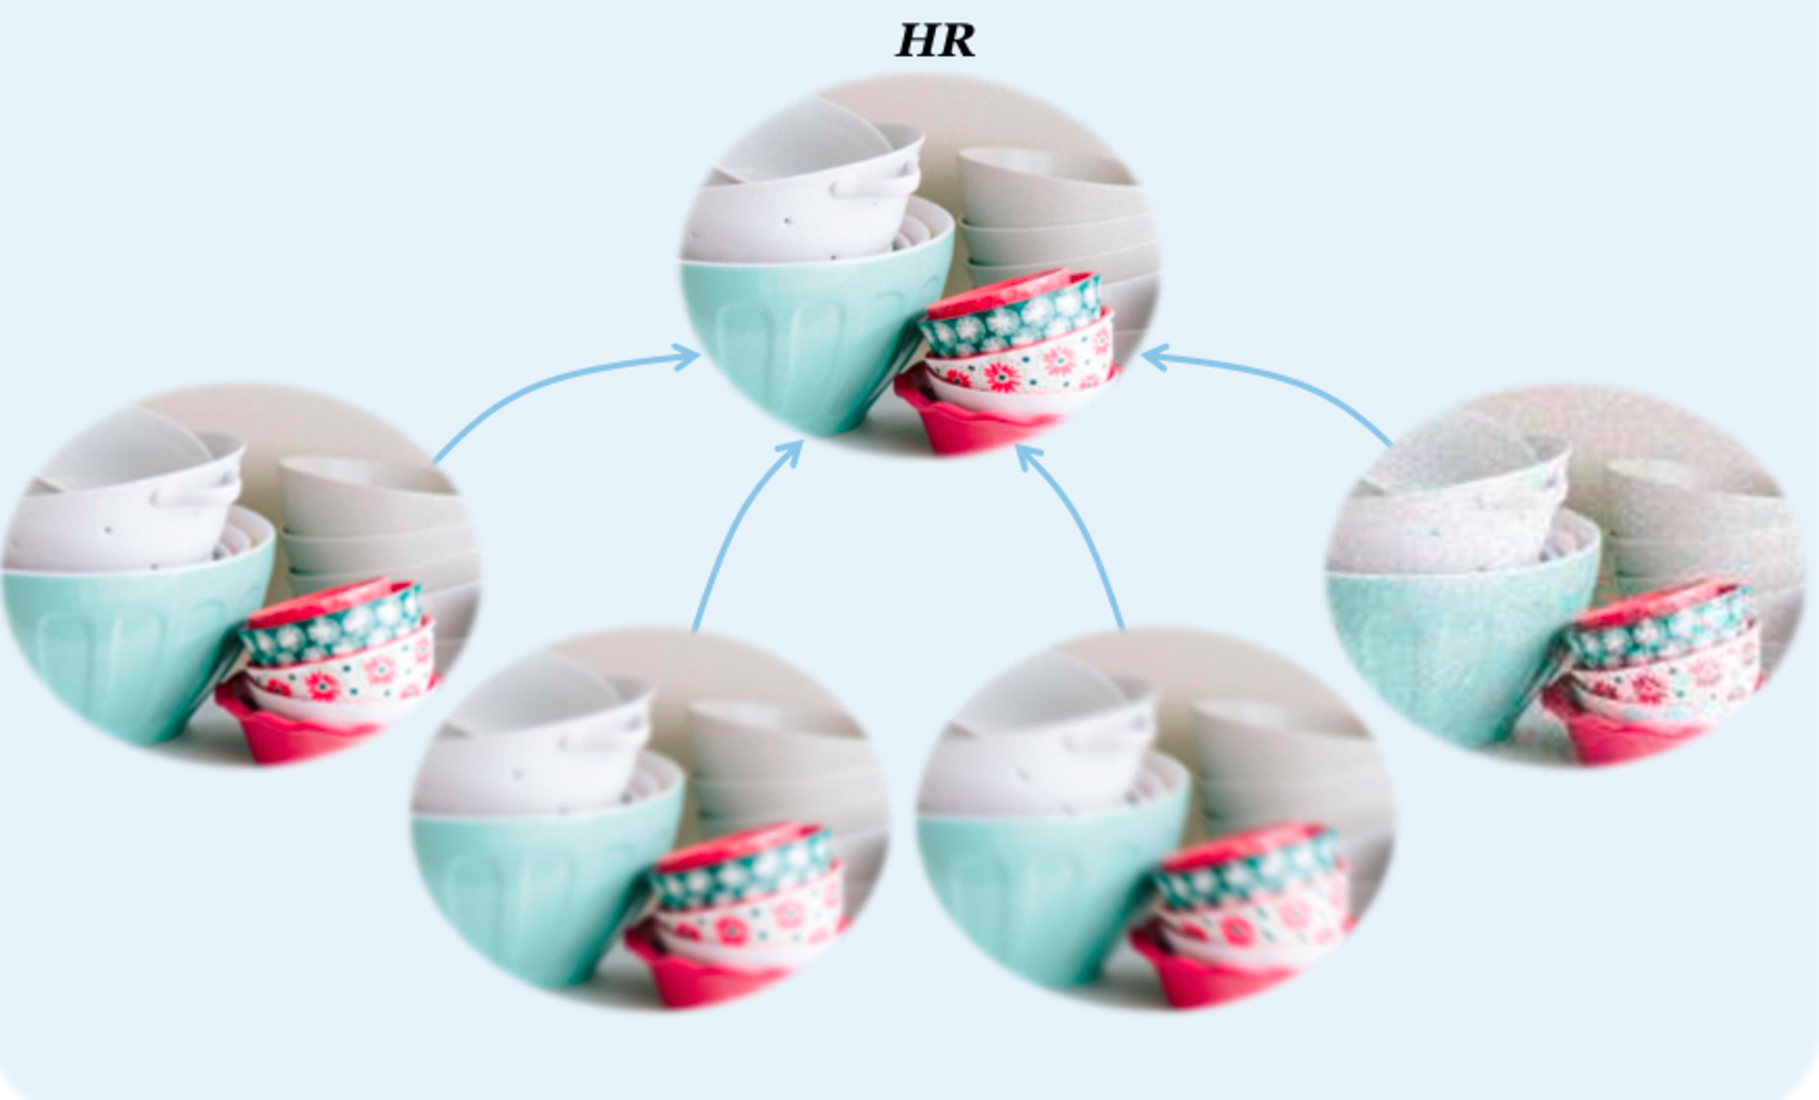
\includegraphics[scale=0.4]{Includes/2-domain-gap.pdf}
            \caption{Effects of different degradation models on one HR image. Source: \cite{liu2021blind}}
            \label{fig:2-domain-gap}
        \end{figure}

            




    \subsection{Blind image Super Resolution}

        The problem of SR with an unknown degradation process is known as blind SR. 
        Growing attention has been paid to blind SR in recent years, towards filling the domain gap presented in \ref{subsec:domaingap}.
        A schematic diagram of the problem is shown in Fig. \ref{fig:2-DomainGap}. 
        Non-blind SR assume that the degradation process is known, and maps the bicubic downsampled LR image to the natural HR image space.
        However, an arbitrary LR input image, as a scene captured by a satellite, is usually degraded by an unknown process, which is difficult to be modelled explicitly.
        The arbitrary LR input is not in the same domain as the bicubic downsamopled LR image, and thus the non-blind SR methods are not successful, moving to a different place in the HR space than the natural images.
        Blind SR methods, on the other hand, aim to learn the degradation process from the training data, and map the arbitrary LR input image to the natural HR image space.

        \begin{figure}[H]
            \centering
            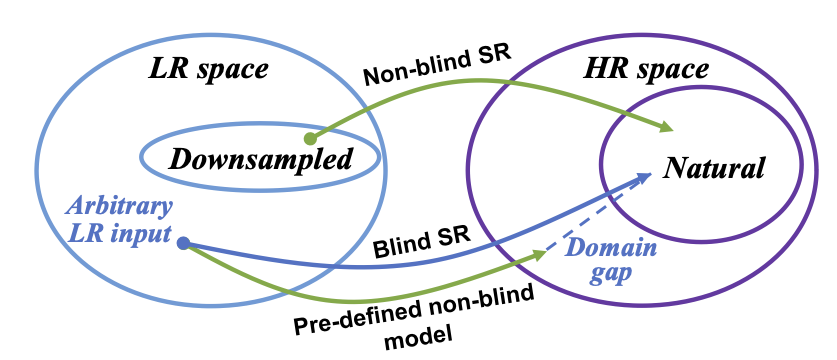
\includegraphics[scale=0.45]{Includes/2-DomainGap.png}
            \caption{Domain interpretation of differences between non-blind and blind SR. Source: \cite{liu2021blind}}
            \label{fig:2-DomainGap}
        \end{figure}


        \begin{figure}[H]
            \centering
            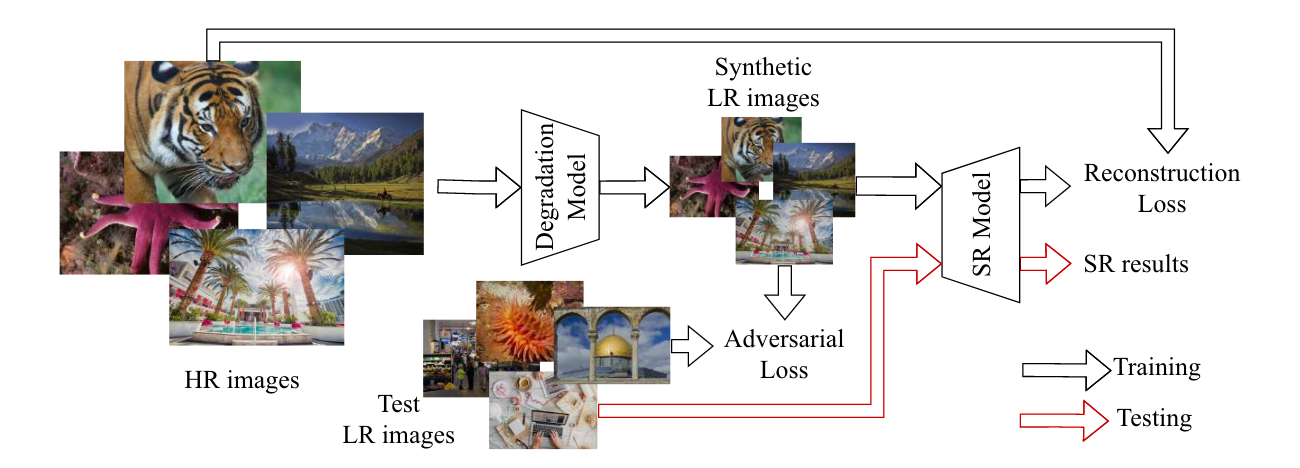
\includegraphics[scale=0.65]{Includes/3-GAN-degradation-model.png}
            \caption{In Degradation-learning-based methods, 
                     adversarial training is used to encourage the degradation model to produce images in the same domain with the target domain (test images).
                     Source \cite{luo2022learning}.}
            \label{fig:3-GAN-degradation-model}
        \end{figure}

        

\clearpage